Author: Lester Hedges Email:~~ lester.hedges@bristol.ac.uk

\hypertarget{molecular-setup}{%
\section{Molecular setup}\label{molecular-setup}}

The companion notebook for this section can be found
\href{https://github.com/michellab/BioSimSpaceTutorials/blob/4844562e7d2cd0b269cead56562ec16a3dfaef7c/01_introduction/02_molecular_setup.ipynb}{here}

\hypertarget{introduction}{%
\subsection{Introduction}\label{introduction}}

In this section we will learn how to use BioSimSpace to set up a
molecular system ready for simulation. Starting from a molecular
topology in the form of a \href{https://www.rcsb.org/}{Protein Data
Bank} format file, we will learn how to parameterise molecules using
different molecular
\href{https://en.wikipedia.org/wiki/Force_field_(chemistry)}{force
fields}, then solvate them using various
\href{https://en.wikipedia.org/wiki/Water_model}{water models}.

\hypertarget{a-note-regarding-molecular-input}{%
\subsubsection{A note regarding molecular
input}\label{a-note-regarding-molecular-input}}

The starting point for many simulations is a molecular topology in the
form of a \href{https://www.rcsb.org/}{PDB} file. This file contains
information regarding the structure of the molecule (its constituent
residues and atoms), the layout of atoms in space (in the form of 3D
atomic coordinates), and sometimes additional molecular information such
as the formal charge of each atom. What this file does not contain is
information describing how the atoms in the molecule \emph{interact},
i.e.~what are the functional forms and parameters for the terms in the
molecular potential. This file is then used as the input to a
\emph{parameterisation engine}, which typically matches the atoms and
residues against templates in order to \emph{parameterise} the molecule
with a chosen force field. As such, the accuracy of the original
topology is of critical importance: Atoms and residues \emph{must} have
the correct names, and the topology \emph{must} be complete, i.e.~no
missing atoms.

Unfortunately, many tools do a poor job in preparing PDB files,
e.g.~having quirks with their naming conventions, excluding certain
atoms, etc. Since it is impossible to account for all such
inconsistencies, which often takes detailed knowledge of the particular
system and tool in question, BioSimSpace takes the approach that the
original files used to create a starting moleular system should be
properly formatted from the outset. We don't want to make guesses as to
what the user intended, or leave them confused if unexpected behaviour
occurs later down the line.

If pre-processing of the PDB file is required, then we recommend using
one of the following third-party tools:

\begin{itemize}
\tightlist
\item
  \href{https://github.com/Amber-MD/pdb4amber}{pdb4amber}
\item
  \href{https://htmlpreview.github.io/?https://github.com/openmm/pdbfixer/blob/master/Manual.html}{PDBFixer}
\end{itemize}

When present, we do provide rudimentary support for \texttt{pdb4amber}
via the \texttt{BioSimSpace.IO.reaadPDB} function, where passing the
\texttt{pdb4amber=True} argument will pre-process the file with
\texttt{pdb4amber} prior to creating a molecular system. However, we
choose only to support the \emph{default} options, since many are
experimental and have can have undesirable knock-on effects, e.g.~using
the \texttt{-\/-add-missing-atoms} option strips all chain identifiers
from the molecule.

\hypertarget{parameterisation}{%
\subsection{Parameterisation}\label{parameterisation}}

The
\href{https://biosimspace.org/api/index_Parameters.html}{BioSimSpace.Parameters}
package provides support for parameterising molecules using three
different engines:

\begin{itemize}
\tightlist
\item
  \href{https://ambermd.org/AmberTools.php}{AmberTools} (Using the
  \texttt{tLEaP} and \texttt{antechamber} programs.)
\item
  \href{https://manual.gromacs.org/documentation/current/onlinehelp/gmx-pdb2gmx.html}{gmx
  pdb2gmx} (Used as a fall-back for certain AMBER force fields when
  AmberTools isn't present.)
\item
  \href{https://github.com/openforcefield/openff-toolkit}{openff-toolkit}
  (The toolkit of the \href{https://openforcefield.org/}{Open Force
  Field Initiative}.)
\end{itemize}

Let's load BioSimSpace and see what force fields are available:

\begin{Shaded}
\begin{Highlighting}[]
\ImportTok{import}\NormalTok{ BioSimSpace }\ImportTok{as}\NormalTok{ BSS}

\NormalTok{BSS.Parameters.forceFields()}
\end{Highlighting}
\end{Shaded}

\begin{verbatim}
['ff03',
 'ff14SB',
 'ff99',
 'ff99SB',
 'ff99SBildn',
 'gaff',
 'gaff2',
 'openff_unconstrained-1.0.0',
 'openff_unconstrained-1.3.0',
 'openff_unconstrained-1.2.0',
 'openff_unconstrained-1.0.1',
 'openff_unconstrained-1.0.0-RC2',
 'openff_unconstrained-1.1.0',
 'openff_unconstrained-1.2.1',
 'openff_unconstrained-1.1.1',
 'openff_unconstrained-1.0.0-RC1']
\end{verbatim}

The supported force fields fall into two categories:

\begin{enumerate}
\def\labelenumi{\arabic{enumi})}
\tightlist
\item
  AMBER force fields:
\end{enumerate}

\begin{Shaded}
\begin{Highlighting}[]
\NormalTok{BSS.Parameters.amberForceFields()}
\end{Highlighting}
\end{Shaded}

\begin{verbatim}
['ff03', 'ff14SB', 'ff99', 'ff99SB', 'ff99SBildn', 'gaff', 'gaff2']
\end{verbatim}

N.B. We currently don't support force fields from \texttt{AmberTools20}
that use CMAP corrections.

\begin{enumerate}
\def\labelenumi{\arabic{enumi})}
\setcounter{enumi}{1}
\tightlist
\item
  Open Force Fields:
\end{enumerate}

\begin{Shaded}
\begin{Highlighting}[]
\NormalTok{BSS.Parameters.openForceFields()}
\end{Highlighting}
\end{Shaded}

\begin{verbatim}
['openff_unconstrained-1.0.0',
 'openff_unconstrained-1.3.0',
 'openff_unconstrained-1.2.0',
 'openff_unconstrained-1.0.1',
 'openff_unconstrained-1.0.0-RC2',
 'openff_unconstrained-1.1.0',
 'openff_unconstrained-1.2.1',
 'openff_unconstrained-1.1.1',
 'openff_unconstrained-1.0.0-RC1']
\end{verbatim}

N.B. We currently don't support the default \emph{constrained} versions
of the force fields, since we require conversion via an intermediate
\href{https://github.com/ParmEd/ParmEd}{ParmEd} topology that needs
explicit bond parameters. If required, constraints can be added at a
later stage. This will hopefully be resolved future releases when direct
translation from Open Force Field to BioSimSpace data structures should
be possible.

N.B. The available Open Force Fields are determined dynamically at
import time, so the list above might be different depending on what
version of the \texttt{openff-toolkit} you have installed.

Let's load a small molecule and parameterise it with several supported
force fields.

\begin{Shaded}
\begin{Highlighting}[]
\CommentTok{# Load a methanol molecule from a PDB file. Since there is only a single}
\CommentTok{# molecule, we take the first item from the system that was created.}
\NormalTok{molecule }\OperatorTok{=}\NormalTok{ BSS.IO.readMolecules(}\StringTok{"inputs/methanol.pdb"}\NormalTok{)[}\DecValTok{0}\NormalTok{]}
\end{Highlighting}
\end{Shaded}

As mentioned above, this is just a bare molecule that only contains
information pertaining to the topology. To see this, we can query the
\emph{properties} of the underlying
\href{https://github.com/michellab/Sire}{Sire} object.

\begin{Shaded}
\begin{Highlighting}[]
\NormalTok{molecule._sire_object.propertyKeys()}
\end{Highlighting}
\end{Shaded}

\begin{verbatim}
['insert_code',
 'beta_factor',
 'coordinates',
 'element',
 'occupancy',
 'formal_charge',
 'fileformat',
 'is_het',
 'alt_loc']
\end{verbatim}

We'll now parameterise the molecule with the
\href{http://ambermd.org/antechamber/gaff.html}{General AMBER force
field}, commonly known as GAFF. Behind the scenes this will set up and
run the
\href{http://ambermd.org/tutorials/basic/tutorial4b/}{antechamber} and
\href{https://ambermd.org/tutorials/pengfei/index.htm}{tLEaP} programs
from the \href{https://ambermd.org/AmberTools.php}{AmberTools} suite.
Depending on the input, \texttt{antechamber} might call out to
\texttt{sqm} to perform a quantum chemistry calculation in order to
calculate charges. Since this can be time consuming for a large
molecule, all of the BioSimSpace parameterisation functions return a
handle to a background process so that you can continue work
interactively while you want for the the parameterisation completes.

\begin{Shaded}
\begin{Highlighting}[]
\NormalTok{process }\OperatorTok{=}\NormalTok{ BSS.Parameters.gaff(molecule)}
\end{Highlighting}
\end{Shaded}

When you're ready to get the molecule, just call \texttt{.getMolecule()}
on the process which will block until the parameterisation is complete,
following which it will return a new molecule with force field
parameters, or raise an exception if something went wrong.

\begin{Shaded}
\begin{Highlighting}[]
\NormalTok{gaff_molecule }\OperatorTok{=}\NormalTok{ process.getMolecule()}
\end{Highlighting}
\end{Shaded}

N.B. If something went wrong, it can be useful look at the intermediate
files within \texttt{process.workDir()} to see what errors were reported
by the various programs that were run. A \texttt{README.txt} file in
this directory will also tell you exactly what commands were run, and in
what order.

Since this was just a small molecule and parameterisation was quick, we
could have just returned the molecule from the process immediately
using:

\begin{Shaded}
\begin{Highlighting}[]
\NormalTok{gaff_molecule }\OperatorTok{=}\NormalTok{ BSS.Parameters.gaff(molecule).getMolecule()}
\end{Highlighting}
\end{Shaded}

N.B. When returning immediately any intermediate files will be lost
unless the \texttt{work\_dir} parameter was used to specify a working
directory for the process.

Once again, we can query the underlying Sire object to see what
properties are associated with the molecule:

\begin{Shaded}
\begin{Highlighting}[]
\NormalTok{gaff_molecule._sire_object.propertyKeys()}
\end{Highlighting}
\end{Shaded}

\begin{verbatim}
['gb_screening',
 'coordinates',
 'charge',
 'formal_charge',
 'angle',
 'forcefield',
 'improper',
 'mass',
 'gb_radius_set',
 'element',
 'alt_loc',
 'dihedral',
 'occupancy',
 'insert_code',
 'connectivity',
 'atomtype',
 'fileformat',
 'treechain',
 'intrascale',
 'beta_factor',
 'gb_radii',
 'is_het',
 'ambertype',
 'bond',
 'LJ']
\end{verbatim}

In addition to the properties loaded from the original PDB file we now
have properties that relate to the force field parameters, such as
\texttt{bond}, \texttt{angle}, and \texttt{dihedral}.

Note that when calling \texttt{.getMolecule()} BioSimSpace copies any
additional properties from the parameterised system (created by loading
the final output from the parameterisation process) back into the a copy
of the original molecule, such that the \emph{original} topology is
\emph{preserved}. For example, while the parameterisation process may
have renamed atoms/residues, or reordered atoms, the naming and ordering
in the returned molecule will match the original that was passed in. As
mentioned earlier, we don't deal with situations where the
parameterisation engine \emph{adds} atoms that were missing from the
original topology. In this case the parameterisation would fail, since
the new topology is inconsistent with the original.

Let us now parameterise the same molecule using one of the Open Force
Fields:

\begin{Shaded}
\begin{Highlighting}[]
\NormalTok{openff_molecule }\OperatorTok{=}\NormalTok{ BSS.Parameters.openff_unconstrained_1_0_0(molecule).getMolecule()}
\end{Highlighting}
\end{Shaded}

We can now loop over atoms in the two parameterised molecules and
compare properties. For example, we can see that the atomic charges are
the same:

\begin{Shaded}
\begin{Highlighting}[]
\ControlFlowTok{for}\NormalTok{ atom0, atom1 }\KeywordTok{in} \BuiltInTok{zip}\NormalTok{(gaff_molecule.getAtoms(), openff_molecule.getAtoms()):}
    \BuiltInTok{print}\NormalTok{(atom0.name(), atom0.charge(), atom1.charge())}
\end{Highlighting}
\end{Shaded}

\begin{verbatim}
C 0.1167 |e| 0.1167 |e|
H1 0.0287 |e| 0.0287 |e|
H2 0.0287 |e| 0.0287 |e|
H3 0.0287 |e| 0.0287 |e|
OH -0.5988 |e| -0.5988 |e|
HO 0.3960 |e| 0.3960 |e|
\end{verbatim}

To compare specific terms in the force field we can query the properties
of the underlying Sire objects:

\begin{Shaded}
\begin{Highlighting}[]
\CommentTok{# Get the bond potentials generated by GAFF.}
\NormalTok{gaff_molecule._sire_object.}\BuiltInTok{property}\NormalTok{(}\StringTok{"bond"}\NormalTok{).potentials()}
\end{Highlighting}
\end{Shaded}

\begin{verbatim}
[TwoAtomFunction( {CGIdx(0),Index(0)} <-> {CGIdx(0),Index(2)} : 330.6 [r - 1.0969]^2 ),
 TwoAtomFunction( {CGIdx(0),Index(0)} <-> {CGIdx(0),Index(3)} : 330.6 [r - 1.0969]^2 ),
 TwoAtomFunction( {CGIdx(0),Index(0)} <-> {CGIdx(0),Index(1)} : 330.6 [r - 1.0969]^2 ),
 TwoAtomFunction( {CGIdx(0),Index(4)} <-> {CGIdx(0),Index(5)} : 371.4 [r - 0.973]^2 ),
 TwoAtomFunction( {CGIdx(0),Index(0)} <-> {CGIdx(0),Index(4)} : 316.7 [r - 1.4233]^2 )]
\end{verbatim}

\begin{Shaded}
\begin{Highlighting}[]
\CommentTok{# Get the bond potentials generated by OpenFF.}
\NormalTok{openff_molecule._sire_object.}\BuiltInTok{property}\NormalTok{(}\StringTok{"bond"}\NormalTok{).potentials()}
\end{Highlighting}
\end{Shaded}

\begin{verbatim}
[TwoAtomFunction( {CGIdx(0),Index(0)} <-> {CGIdx(0),Index(2)} : 379.047 [r - 1.09289]^2 ),
 TwoAtomFunction( {CGIdx(0),Index(0)} <-> {CGIdx(0),Index(3)} : 379.047 [r - 1.09289]^2 ),
 TwoAtomFunction( {CGIdx(0),Index(0)} <-> {CGIdx(0),Index(1)} : 379.047 [r - 1.09289]^2 ),
 TwoAtomFunction( {CGIdx(0),Index(4)} <-> {CGIdx(0),Index(5)} : 560.292 [r - 0.970769]^2 ),
 TwoAtomFunction( {CGIdx(0),Index(0)} <-> {CGIdx(0),Index(4)} : 334.571 [r - 1.41429]^2 )]
\end{verbatim}

As well as being able to parameterise a molecule loaded from file,
BioSimSpace can also use a
\href{https://en.wikipedia.org/wiki/Simplified_molecular-input_line-entry_system}{SMILES}
string as the molecule parameter for any force field function. This can
be useful if you want to highlight particular steroechemistry, which
might not be possible in the intermediate file formats that are used
behind the scenes duing the parameterisation, e.g.~PDB. When using
SMILES there is no constraint that the parameterised topology matches
that of the original molecule, since we have not yet created a
fully-fledged BioSimSpace molecule at the point at which we invoke the
parameterisation. As such, it is perfectly acceptable for the
parameterisation to add hydrogen atoms.

With this in mind, the two parameterisations shown above could also have
been performed as follows:

\begin{Shaded}
\begin{Highlighting}[]
\NormalTok{gaff_molecule }\OperatorTok{=}\NormalTok{ BSS.Parameters.gaff(}\StringTok{"CO"}\NormalTok{).getMolecule()}
\NormalTok{openff_molecule }\OperatorTok{=}\NormalTok{ BSS.Parameters.openff_unconstrained_1_0_0(}\StringTok{"CO"}\NormalTok{).getMolecule()}
\end{Highlighting}
\end{Shaded}

Here hydrogen atoms have been added during the parameterisation. While
the atom layout and naming is different those of the previous examples,
the parameters for the equivalent atoms are the same, e.g.:

\begin{Shaded}
\begin{Highlighting}[]
\ControlFlowTok{for}\NormalTok{ atom0, atom1 }\KeywordTok{in} \BuiltInTok{zip}\NormalTok{(gaff_molecule.getAtoms(), openff_molecule.getAtoms()):}
    \BuiltInTok{print}\NormalTok{(atom0.name(), atom0.charge(), atom1.charge())}
\end{Highlighting}
\end{Shaded}

\begin{verbatim}
C1 0.1167 |e| 0.1167 |e|
O1 -0.5988 |e| -0.5988 |e|
H1 0.0287 |e| 0.0287 |e|
H2 0.0287 |e| 0.0287 |e|
H3 0.0287 |e| 0.0287 |e|
H4 0.3960 |e| 0.3960 |e|
\end{verbatim}

In addition to small molecules, BioSimSpace provides support for
parameterising proteins using force fields from \texttt{AmberTools},
such as
\href{https://pubs.acs.org/doi/abs/10.1021/acs.jctc.5b00255}{ff14SB}.
(We don't currently support
\href{https://pubs.acs.org/doi/10.1021/acs.jctc.9b00591}{ff19SB} due to
the presence of CMAP terms, which we don't yet support in our parsers.)

As an example:

\begin{Shaded}
\begin{Highlighting}[]
\NormalTok{protein }\OperatorTok{=}\NormalTok{ BSS.IO.readMolecules(}\StringTok{"inputs/2JJC.pdb"}\NormalTok{)[}\DecValTok{0}\NormalTok{]}
\NormalTok{protein }\OperatorTok{=}\NormalTok{ BSS.Parameters.ff14SB(protein).getMolecule()}
\end{Highlighting}
\end{Shaded}

When molecules contain bound ions it is necessary to choose a water
model for the ion parameters. This can be achieved by passing the
\texttt{water\_model} argument to any parameterisation function, where
the named water model must match one of those described in the
\textbf{Solvation} section below, e.g. \texttt{water\_model="tip3p"}.
(An exception will be raised if bound ions are detected and no water
model is chosen.) An optional \texttt{leap\_commands} argument allows
you to pass additional directives to the \texttt{tLEaP} program called
by an AMBER protein force field function. These commands are added after
the defaults allowing you to load custom force field parameters, etc.

\hypertarget{solvation}{%
\subsection{Solvation}\label{solvation}}

The next stage in setting up a system ready for simulation is to solvate
the molecule(s) in a box of water. The
\href{https://biosimspace.org/api/index_Solvent.html}{BioSimSpace.Solvent}
package provides support for solvating with a variety of water models:

\begin{Shaded}
\begin{Highlighting}[]
\NormalTok{BSS.Solvent.waterModels()}
\end{Highlighting}
\end{Shaded}

\begin{verbatim}
['spc', 'spce', 'tip3p', 'tip4p', 'tip5p']
\end{verbatim}

N.B. At present we only support solvating in water.

Solvation is performed using the
\href{https://manual.gromacs.org/documentation/2018/onlinehelp/gmx-solvate.html}{gmx
solvate} package. We currently don't support other solvation engines,
since they require parameterisation as a pre-requisite, or include
parameterisation as part of the solvation process itself, i.e.~you can't
decouple the two stages. We will hopefully overcome this shortcoming in
future releases, since other engines would enable support for
\href{https://www.ncbi.nlm.nih.gov/pmc/articles/PMC6078207/}{more
realistic salt concentrations} and improved water templates, i.e.~less
vapour bubbles at box edges, which need to be properly equlibrated.

BioSimSpace provides support for both orthorhombic and triclinic
simulation boxes, where appropriate box magnitudes and angles can be
obtained using the
\href{https://biosimspace.org/api/index_Box.html}{BioSimSpace.Box}
package. To see what pre-generated box types are available:

\begin{Shaded}
\begin{Highlighting}[]
\NormalTok{BSS.Box.boxTypes()}
\end{Highlighting}
\end{Shaded}

\begin{verbatim}
['cubic',
 'rhombicDodecahedronHexagon',
 'rhombicDodecahedronSquare',
 'truncatedOctahedron']
\end{verbatim}

For example, to get box parameters for a truncated octahedral box with
an image distance of 10 nanometers.

\begin{Shaded}
\begin{Highlighting}[]
\NormalTok{box, angles }\OperatorTok{=}\NormalTok{ BSS.Box.truncatedOctahedron(}\DecValTok{10}\OperatorTok{*}\NormalTok{BSS.Units.Length.nanometer)}
\BuiltInTok{print}\NormalTok{(box, angles)}
\end{Highlighting}
\end{Shaded}

\begin{verbatim}
[100.0000 A, 100.0000 A, 100.0000 A] [109.4712 degrees, 70.5288 degrees, 70.5288 degrees]
\end{verbatim}

When choosing a box for solvation it is important to ensure that it
large enough to hold the molecule(s) of interest. In addition, when
adding ions to neutralise the system or reach a desired ionic strength,
then the system must be large enough that the cut-off used by
\href{https://manual.gromacs.org/archive/5.0/programs/gmx-genion.html}{gmx
genion} when computing electrostatics is not more than twice the
shortest box dimension. This can lead to a slight self-consistency
issue, since it's sometimes not possible to know the number of ions that
will need to be added a priori. Even if that were possible, then the
random insertion of ions by \texttt{gmx\ genion} can still lead to
issues if the choice of location means that they don't all manage to fit
within the available volume.

As such, sometimes a little trial-and-error is needed to find an
appropriate box size for the system in question. A good rule of thumb is
to obtain the
\href{https://en.wikipedia.org/wiki/Bounding_volume}{axis-aligned
bounding box} for the molecule(s) and add an appropriate buffer to the
largest box dimension. For example:

\begin{Shaded}
\begin{Highlighting}[]
\CommentTok{# Get the minimium and maximum coordinates of the bounding box that}
\CommentTok{# minimally encloses the protein.}
\NormalTok{box_min, box_max }\OperatorTok{=}\NormalTok{ protein.getAxisAlignedBoundingBox()}

\CommentTok{# Work out the box size from the difference in the coordinates.}
\NormalTok{box_size }\OperatorTok{=}\NormalTok{ [y }\OperatorTok{-}\NormalTok{ x }\ControlFlowTok{for}\NormalTok{ x, y }\KeywordTok{in} \BuiltInTok{zip}\NormalTok{(box_min, box_max)]}

\CommentTok{# How much to pad each side of the protein? (Nonbonded cutoff = 10 A)}
\NormalTok{padding }\OperatorTok{=} \DecValTok{15} \OperatorTok{*}\NormalTok{ BSS.Units.Length.angstrom}

\CommentTok{# Work out an appropriate box. This will used in each dimension to ensure}
\CommentTok{# that the cutoff constraints are satisfied if the molecule rotates.}
\NormalTok{box_length }\OperatorTok{=} \BuiltInTok{max}\NormalTok{(box_size) }\OperatorTok{+} \DecValTok{2}\OperatorTok{*}\NormalTok{padding}
\end{Highlighting}
\end{Shaded}

Armed with this information, we can now solvate our protein in an
appropriately sized cubic box. Here we will use the TIP3P water model:

\begin{Shaded}
\begin{Highlighting}[]
\NormalTok{solvated }\OperatorTok{=}\NormalTok{ BSS.Solvent.tip3p(molecule}\OperatorTok{=}\NormalTok{protein, box}\OperatorTok{=}\DecValTok{3}\OperatorTok{*}\NormalTok{[box_length])}
\end{Highlighting}
\end{Shaded}

N.B. The \texttt{molecule} argument is optional. If ommited, then a pure
water box will be generated.

By default, BioSimSpace will add counter-ions to neutralise the system.
To see what ions were added we can use the built in \texttt{search}
functionality:

\begin{Shaded}
\begin{Highlighting}[]
\CommentTok{# Search for all free ions. As a simple search, we look for all molecules}
\CommentTok{# that only contain a single atom.}
\NormalTok{search }\OperatorTok{=}\NormalTok{ solvated.search(}\StringTok{"not mols with atomidx 2"}\NormalTok{)}

\CommentTok{# Print all ions and their charge.}
\ControlFlowTok{for}\NormalTok{ ion }\KeywordTok{in}\NormalTok{ search:}
    \BuiltInTok{print}\NormalTok{(}\SpecialStringTok{f"element = }\SpecialCharTok{\{}\NormalTok{ion}\SpecialCharTok{.}\NormalTok{element()}\SpecialCharTok{\}}\SpecialStringTok{, charge = }\SpecialCharTok{\{}\NormalTok{ion}\SpecialCharTok{.}\NormalTok{charge()}\SpecialCharTok{\}}\SpecialStringTok{"}\NormalTok{)}
\end{Highlighting}
\end{Shaded}

\begin{verbatim}
element = Sodium (Na, 11), charge = 1.0000 |e|
element = Sodium (Na, 11), charge = 1.0000 |e|
element = Sodium (Na, 11), charge = 1.0000 |e|
element = Sodium (Na, 11), charge = 1.0000 |e|
element = Sodium (Na, 11), charge = 1.0000 |e|
element = Sodium (Na, 11), charge = 1.0000 |e|
element = Sodium (Na, 11), charge = 1.0000 |e|
\end{verbatim}

He're we see that \texttt{gmx\ genion} added 7 sodium ions. To confirm
that the system was indeed neutralised, we can check its charge, as well
as the charge of the original protein:

\begin{Shaded}
\begin{Highlighting}[]
\BuiltInTok{print}\NormalTok{(}\SpecialStringTok{f"solvated = }\SpecialCharTok{\{}\NormalTok{solvated}\SpecialCharTok{.}\NormalTok{charge()}\SpecialCharTok{\}}\SpecialStringTok{, protein = }\SpecialCharTok{\{}\NormalTok{protein}\SpecialCharTok{.}\NormalTok{charge()}\SpecialCharTok{\}}\SpecialStringTok{"}\NormalTok{)}
\end{Highlighting}
\end{Shaded}

\begin{verbatim}
solvated = -1.2183e-07 |e|, protein = -7.0000 |e|
\end{verbatim}

We now have a solvated system ready for simulation. Let's visualise it
with
\href{https://biosimspace.org/api/generated/BioSimSpace.Notebook.View.html\#BioSimSpace.Notebook.View}{BioSimSpace.Notebook.View}:

\begin{Shaded}
\begin{Highlighting}[]
\NormalTok{view }\OperatorTok{=}\NormalTok{ BSS.Notebook.View(solvated)}
\NormalTok{view.system()}
\end{Highlighting}
\end{Shaded}

\begin{figure}
\centering
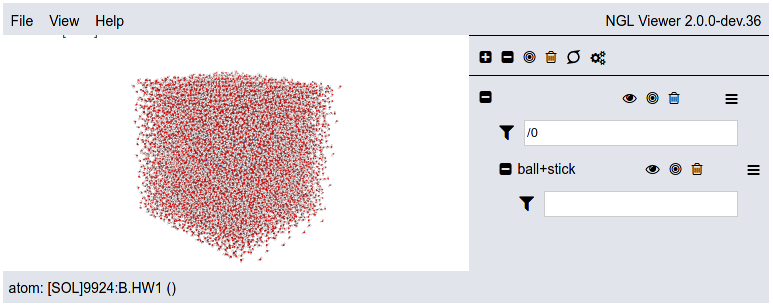
\includegraphics{https://github.com/michellab/BioSimSpaceTutorials/blob/d26d5bcfe8e66fa6c9aa8bdb9788fb5eeb252ee8/01_introduction/assets/02_solvated.png}
\caption{Visualisation of the solvated system.}
\end{figure}

Finally, let's save the system to file in AMBER format.

\begin{Shaded}
\begin{Highlighting}[]
\NormalTok{BSS.IO.saveMolecules(}\StringTok{"solvated"}\NormalTok{, solvated, [}\StringTok{"prm7"}\NormalTok{, }\StringTok{"rst7"}\NormalTok{])}
\end{Highlighting}
\end{Shaded}

\begin{verbatim}
['/home/lester/Code/BioSimSpaceTutorials/01_introduction/solvated.prm7',
 '/home/lester/Code/BioSimSpaceTutorials/01_introduction/solvated.rst7']
\end{verbatim}
